\documentclass{beamer}
\usepackage[english]{babel}

\usepackage{lipsum}
\usepackage{todonotes}
\usepackage{style}
\usepackage{tabularx}
\usepackage{hyperref}

% Theme based on https://github.com/elauksap/beamerthemepolimi
\usetheme[bgphoto]{polimi}
\usefonttheme[onlymath]{serif}

\setbeamertemplate{bibliography item}{\insertbiblabel}

% Hide section name from frame header
\newif\ifhidesechead
\hidesecheadfalse

\title{\tlap}
\subtitle{%
    A modeling language for
    \texorpdfstring{\linebreak}{}%
    concurrent and distributed systems
}
\author{M. Donadoni \and A. Fulgini \and E. Morassutto}

\begin{document}
    \begin{frame}
        \maketitle
    \end{frame}

    \begin{frame}{Table of contents}
      \tableofcontents[hideallsubsections]
    \end{frame}

    \section[image=bgphoto_cut]{Introduction}
\begin{frame}[plain]{}
    \sectionpage
\end{frame}

\begin{frame}{\tlap}
    \tlap is a high-level specification language for modeling concurrent and distributed digital systems:
    \begin{itemize}
        \item Algorithms
        \item Programs
        \item Complex computing systems
    \end{itemize}

    \tlap is based on set theory, first-order logic and the Temporal Logic of Actions (TLA); it uses ordinary, basic math.
\end{frame}

\begin{frame}{Leslie Lamport}
    \tlap is developed by Leslie Lamport
    \begin{itemize}
        \item Original author of \LaTeX, first release in 1984
        \item Fundamental contribution to the theory of distributed systems
        \begin{itemize}
            \item Logical Clocks
            \item Byzantine General's problem
            \item Chandy-Lamport distributed snapshot algorithm
            \item Paxos algorithm
            \item many, many other contributions
        \end{itemize}
        \item Turing Award in 2013 (and many other prizes)
    \end{itemize}
\end{frame}

\begin{frame}{\tlap tooling}
    \setbeamercovered{transparent}
    \begin{description}
        \item<1->[\tlap] specification language
        \item<1->[TLC] model checker and simulator of \tlap specs
        \item<-1>[PlusCal] algorithm language similar to a simple programming language, can be translated to \tlap
        \item<-1>[TLAPS] system for mechanically checking proofs written in \tlap
        \item<-1>[TLATeX] pretty-printer to typeset \tlap specifications in \LaTeX
        \item<1->[Toolbox] IDE for all the \tlap tools
    \end{description}
    \setbeamercovered{invisible}
    \pause
    \vspace{0.5cm}
    \begin{center}
        We will focus on \tlap and TLC and we will use the \tlap Toolbox
    \end{center}
\end{frame}

%TODO: history?

\begin{frame}{Motivations for simple, high-level language}
    Why should we use an high-level language which uses ordinary and simple math instead of some kind of programming language?
    \setbeamercovered{transparent}
    \begin{itemize}[<+->]
        \item It helps us abstract away from implementation details
        \item No special or new syntax, only simple math
        \item Specification of the system is written before the implementation, design errors are found as early as possible
        \item Specification is independent from the language used for implementation
    \end{itemize}
    \setbeamercovered{invisible}
\end{frame}

\begin{frame}{Industrial use of \tlap}
    Who uses \tlap?
    \setbeamercovered{transparent}
    \begin{itemize}
        \item<1> Intel
        \only<1>{
            \begin{itemize}
                \item Used since 2002
                \item Pre-RTL formal verification of cache-coherence protocol %TODO bib
            \end{itemize}
        }
        \item<2> Microsoft
        \only<2>{
            \begin{itemize}
                \item Used since 2004; usage increased in 2015 due to Azure
                \item Found subtle bugs in memory coherence protocol of Xbox 360, Cosmos DB, lock-free data structures
                \item Public specification of the consistency levels of Cosmos DB %TODO link to repo
            \end{itemize}
        }
        \item<3> OpenComRTOS
        \only<3>{
            \begin{itemize}
                \item New version of \emph{Virtuoso}, the OS of the European Space Agency's \emph{Rosetta} spacecraft
                \item \tlap specification helped to have a cleaner architecture, achieving 10x less code than Virtuoso %TODO bib
            \end{itemize}
        }
        \item<4> Amazon
        \only<4>{
            \begin{itemize}
                \item Used since 2011 for AWS (Amazon Web Services)
                \item As of 2014, used in 10 large complex systems %TODO bib
            \end{itemize}
        }
    \end{itemize}
    \setbeamercovered{invisible}
\end{frame}

\begin{frame}[plain]{Amazon}
    \begin{figure}
        \includegraphics[width=0.9\textwidth]{images/amazon.png}
        \caption{\footnotesize Examples of \tlap usage at Amazon, from} %TODO bib
    \end{figure}
\end{frame}

\section[image=bgphoto_cut]{TLC}
\begin{frame}[plain]{}
    \sectionpage
\end{frame}

\begin{frame}{Specification}
    TLC can evaluate specifications that have the standard form
    \[
        Init \land \square \left[ Next \right]_{vars} \land Temporal
    \]

    where
    \begin{itemize}
        \item $Init$ is the initial predicate
        \item $Next$ is the next-state action
        \item $Temporal$ is a temporal formula (usually liveness conditions)
    \end{itemize}

\end{frame}

\begin{frame}{Temporal Formula}
    TLC can evaluate a temporal formula if it is a conjunction of the following classes of formulas:
    \begin{itemize}
        \item State Predicate
        \item Invariant ( $\square P$, where $P$ is state a predicate)
        \item Box-Action formula ($\square[A]_v$, where $A$ is an action)
        \item Simple Temporal Formula
    \end{itemize}
\end{frame}

\begin{frame}{Simple Temporal Formula}
    Given
    \begin{itemize}
        \item Simple boolean operators ($\land$, $\lor$, $\neg$, $\implies$, $\equiv$, $TRUE$, $FALSE$)
        \item Temporal state formula, that is a temporal formula obtained from state predicates by applying
        \begin{itemize}
            \item simple boolean operators
            \item temporal operators ($\square$, $\Diamond$, $\leadsto$)
        \end{itemize}
        \item Simple action formula\begin{align*}
            \WF_v \left( A \right) &&
            \SF_v \left( A \right) &&
            \square \Diamond \left< A \right>_v &&
            \Diamond \square \left[ A \right]_v &&
        \end{align*}
    \end{itemize}
    A simple temporal formula is defined as a formula constructed from temporal state formulas and simple action formulas by applying simple boolean operators
\end{frame}

\begin{frame}{TLC modes}
    TLC has two different modes
    \setbeamercovered{transparent}
    \begin{itemize}
        \item<1,3> Model-checking mode
        \only<1> {
            \begin{enumerate}
                \item TLC computes all the initial states by evaluating $Init$
                \item TLC constructs the graph of all states of the system, using a BFS, by evaluating $Next$
                \item While expanding the graph, TLC checks that invariants and constraints are satisfied
                \item TLC checks that the temporal properties are satisfied
            \end{enumerate}
        }
        \item<2-> Simulation mode
        \only<2>{
            \begin{itemize}
                \item TLC repeatedly constructs and checks behaviors of the system that have a fixed maximum length
            \end{itemize}
        }
    \end{itemize}
    \setbeamercovered{invisible}
    \only<3>{
        Note that model-checking is possible only if the graph of the states is finite. If it is not finite, constraints to limit the number of states to be considered by TLC can be specified.
    }
\end{frame}

    \section[image=bgphoto_cut]{First Modelling Example}
\begin{frame}[plain]{}
    \sectionpage
\end{frame}

\begin{frame}{Modelling a Clock}
    A \textbf{Clock} is a device with 2 hands:
    \begin{itemize}
        \item The hours one, from 0 to 23
        \item The minutes one, from 0 to 59
    \end{itemize}
    \pause
    The clock should start at 00:00.
    \pause
    \begin{itemize}
        \item After the minutes hand reaches 59, it goes back to 0 and the hours one is incremented.
        \item After the hours hand reaches 23, it goes back to 0.
    \end{itemize}
\end{frame}

\begin{frame}{Modelling variables}
    We need to define 2 variables:
    \pause
    \begin{itemize}[<+->]
        \item \texttt{hr} -- The current hour of the clock
        \item \texttt{min} -- The current minute of the clock
    \end{itemize}
    \onslide<+->
    The only valid initial state for the clock is
    \[
        \texttt{hr} = 0 \quad \land \quad \texttt{min} = 0
    \]
\end{frame}

\begin{frame}{Modelling transitions}
    \begin{block}{Next minute}
        The next minute (\texttt{min'}) is the current one (\texttt{min}) plus one. Buf if the minute is already 59, the next is 0.
    \end{block}
    \pause
    \begin{block}{Next hour}
        \only<2>{
            \texttt{hr' = hr + 1}\\
            \texttt{\phantom{lol}}\\
            \texttt{\phantom{lol}}\\
            \texttt{\phantom{lol}}\\
            \texttt{\phantom{lol}}\\
        }
        \only<3>{
            \texttt{hr' = IF min < 59}\\
            \texttt{\phantom{hr' = }THEN hr}\\
            \texttt{\phantom{hr' = }ELSE hr + 1}\\
            \texttt{\phantom{lol}}\\
            \texttt{\phantom{lol}}\\
        }
        \only<4->{
            \texttt{hr' = IF min < 59}\\
            \texttt{\phantom{hr' = }THEN hr}\\
            \texttt{\phantom{hr' = }ELSE IF hr < 23}\\
            \texttt{\phantom{hr' = ELSE }THEN hr + 1}\\
            \texttt{\phantom{hr' = ELSE }ELSE 0}
        }
    \end{block}
    \onslide<5->
    \begin{block}{Next Predicate}
        \texttt{Next == NextMin $\land$ NextHr}
    \end{block}
\end{frame}

\begin{frame}{Behavior Specification}
    \begin{block}{Option \#1: Init-Next Predicates}
        The model is defined via the predicate for the initial states (\texttt{Init}), and a predicate for the \emph{next} relation (\texttt{Next}).
    \end{block}
    \pause
    \begin{block}{Option \#2: Temporal Formula}
        Specify the behavior using a temporal formula:

        \[
            \texttt{Init} \land \square \texttt{[Next]}_{\texttt{vars}}
        \]
    \end{block}
\end{frame}

\begin{frame}{Check Temporal Formulae}
    We want to verify some temporal formulae:
    \begin{itemize}
        \item The clock always ticks
        \item All the possible times are reachable
    \end{itemize}
    \pause
    \begin{block}{The clock always ticks}
        \[
            \texttt{AlwaysTick == } \square \Diamond \texttt{Next}_{\texttt{vars}}
        \]
    \end{block}
    \pause
    \begin{block}{All the possible times are reachable}
        \begin{equation*}
            \begin{gathered}
                \texttt{AllTimes == } \forall h \in (0 \ldots 23), m \in (0 \ldots 59):\\
                \square \Diamond (\texttt{hr = } h\; \land\; \texttt{min = } m)
            \end{gathered}
        \end{equation*}
    \end{block}
\end{frame}

\begin{frame}{Fixing the Specification}
    Indeed the specified model is not entirely correct:
    \[
        \texttt{00:00} \rightarrow \texttt{00:00} \rightarrow \texttt{00:00} \rightarrow \texttt{00:00} \rightarrow \cdots
    \]
    is a valid behavior composed of an infinite sequence of \emph{stuttering steps}.
    \pause
    We need to add a fairness constraint
    \begin{block}{Weak Fairness constraint}
        \[
            \texttt{LSpec == Clock } \land \texttt{ WF}_{\texttt{vars}}\texttt{(Next)}
        \]
    \end{block}
\end{frame}


    
\section[image=bgphoto_cut]{TLC}
\begin{frame}[plain]{}
    \sectionpage
\end{frame}

\begin{frame}{Specification}
    TLC is an explicit-state model checker for \tlap specifications.
    TLC can evaluate specifications that have the standard form
    \[
        Init \land \square \left[ Next \right]_{vars} \land Temporal
    \]

    where
    \begin{itemize}
        \item $Init$ is the initial predicate
        \item $Next$ is the next-state action
        \item $Temporal$ is a temporal formula (usually liveness conditions)
    \end{itemize}

\end{frame}

\begin{frame}{Temporal Formula}
    TLC can evaluate a temporal formula if it is a conjunction of the following classes of formulas:
    \begin{itemize}
        \item State Predicate
        \item Invariant ($\square P$, where $P$ is state a predicate)
        \item Box-Action formula ($\square[A]_v$, where $A$ is an action)
        \item Simple Temporal Formula
    \end{itemize}
\end{frame}

\begin{frame}{Simple Temporal Formula}
    Given
    \begin{itemize}
        \item Simple boolean operators ($\land$, $\lor$, $\neg$, $\implies$, $\equiv$, $TRUE$, $FALSE$)
        \item Temporal state formula, that is a temporal formula obtained from state predicates by applying
        \begin{itemize}
            \item simple boolean operators
            \item temporal operators ($\square$, $\Diamond$, $\leadsto$)
        \end{itemize}
        \item Simple action formula\begin{align*}
            \WF_v \left( A \right) &&
            \SF_v \left( A \right) &&
            \square \Diamond \left< A \right>_v &&
            \Diamond \square \left[ A \right]_v &&
        \end{align*}
    \end{itemize}
    A simple temporal formula is defined as a formula constructed from temporal state formulas and simple action formulas by applying simple boolean operators
\end{frame}

\begin{frame}{TLC modes}
    TLC has two different modes
    \setbeamercovered{transparent}
    \begin{itemize}
        \item<1,3> Model-checking mode
        \only<1> {
            \begin{enumerate}
                \item TLC computes all the initial states by evaluating $Init$
                \item TLC constructs the graph of all states of the system, using a BFS, by evaluating $Next$
                \item While expanding the graph, TLC checks that invariants and constraints are satisfied
                \item TLC checks that the temporal properties are satisfied
            \end{enumerate}
        }
        \item<2-> Simulation mode
        \only<2>{
            \begin{itemize}
                \item TLC repeatedly constructs and checks behaviors of the system that have a fixed maximum length
            \end{itemize}
        }
    \end{itemize}
    \setbeamercovered{invisible}
    \only<3>{
        Note that model-checking is possible only if the graph of the states is finite. If it is not finite, constraints to limit the number of states to be considered by TLC can be specified.
    }
\end{frame}


    \section[image=trams]{Two-phase commit}
\begin{frame}[plain]{}
    \sectionpage
\end{frame}

\begin{frame}
    \frametitle{Specifying two-phase commit}

    Our goal is to model a system with one \alert{transaction manager} and
    several \alert{resource managers} that need to perform a distributed
    transaction.
    The transaction may:
    \begin{itemize}
        \item \textbf{commit} if all resource managers have committed
        \item \textbf{abort} in any other case
    \end{itemize}

    \begin{center}
        \begin{tikzpicture}[
            >=stealth,
            edge from parent/.style={draw,<->},
            every node/.style={ellipse,draw}
        ]
            \node[rectangle, inner sep=.75em] (tm) {$tm$}
            child foreach \x in {rm1,rm2,rm3} {
                node {$\x$}
            };
        \end{tikzpicture}
    \end{center}
\end{frame}



\subsection{TCommit}
\begin{frame}
    \frametitle{Specifying transaction commit}
    We start with a simple setting, in which we only consider the
    \alert{resource managers} and their \alert{states}.
    We do \emph{not} model
    \begin{itemize}
        \item the transaction manager
        \item the communication channels
        \item the transaction itself
    \end{itemize}
    \uncover<2->{
    We write the specification in module $TCommit$, which will be refined later

    \begin{center}
        \begin{tlatex}
            \moduleLeftDash{ {\MODULE} $TCommit$}\moduleRightDash
        \end{tlatex}
    \end{center}
    }
\end{frame}

\setbeamercovered{transparent}

\begin{frame}
    \frametitle{Constants and variables}

    We declare $RM$ as the set of all resource managers and $rmState$ as the
    state of each resource manager.
    \begin{tlabox}
        &\CONSTANT RM \\
        &\VARIABLE rmState
    \end{tlabox}

    Every constant value is a set -- even 0, 1 and the string "xyz" --
    but for the former their elements are simply undefined, so we
    can't test if $a \in 0$.

    We will assign elements to $RM$ when performing model checking.
\end{frame}

\begin{frame}
    \frametitle{Type checking}
    \begin{uncoverenv}<1>
        \tlap doesn't provide explicit typing of variables. It is customary to
        define an invariant $TypeOK$ to specify the \alert{domain} of each variable.
    \end{uncoverenv}
    \begin{uncoverenv}<2>
        We specify that $rmState$ is an array indexed by $RM$ with values in
        the set of strings below.
    \end{uncoverenv}
    \begin{uncoverenv}<2->
        \begin{tlabox}
            TCTypeOK \defeq rmState \in
            [RM \rightarrow \{&\str{working}, \str{prepared}, \\
                            &\str{committed},\str{aborted}\}]
        \end{tlabox}
    \end{uncoverenv}
    \begin{uncoverenv}<3>
        You can think of it as a mathematical function
        \[
            rmState: RM \rightarrow \{\str{working}, \dots\}
        \]
        We can refer to a value with $rmState[r]$, where $r \in
        RM$.
    \end{uncoverenv}
\end{frame}

\begin{frame}
    \frametitle{The temporal formula of the specification}
    \begin{uncoverenv}<1->
            We specify the behavior with a temporal formula
        \begin{tlabox}
            TCSpec \defeq TCInit \land \Box [TCNext\,]_{rmState}
        \end{tlabox}
    \end{uncoverenv}
    \begin{uncoverenv}<1->
        where initially each resource manager is working
        \begin{tlabox}
            TCInit \defeq [ r \in RM \mapsto \str{working}]
        \end{tlabox}
        and at each step either all resource managers remain in their
        current state (stuttering step) or they take a $Next$-step
    \end{uncoverenv}
\end{frame}

\begin{frame}
    \frametitle{Evolution of the system}

    \begin{columns}[c]
    \begin{column}{0.65\textwidth}
        \uncover<1>{What is a possible step of our system?}

        \uncover<2,3>{A resource manager may}
        \begin{itemize}
            \item<2> Finish working and become prepared
            \item<3> Decide to commit or abort
        \end{itemize}
    \end{column}
    \begin{column}{0.35\textwidth}
        \centering
        \scalebox{.75}{
            \begin{tikzpicture}[
                >=stealth,
                sibling distance=7em,
                edge from parent/.style={draw,->},
                every node/.style={ellipse,draw}
            ]
                \node (w) {$working$}
                child {
                    node (p) {$prepared$}
                    child {
                        node[inner xsep=0] (c) {$committed$}
                    }
                    child {
                        node (a) {$aborted$}
                    }
                };
                \path [draw, ->] (w.south east) to [bend left=30] (a.north);
            \end{tikzpicture}
        }
    \end{column}
    \end{columns}
    \vspace{\baselineskip}
    \begin{tlabox}
        TCNext \defeq \uncover<2,3>{\E r \in RM :}
        \uncover<2>{Prepare(r\,)} \uncover<3>{\lor Decide(r\,)}
    \end{tlabox}
\end{frame}

\begin{frame}
    \frametitle{The Prepare action}

    Resource manager $r$ evolves from \str{working} to \str{prepared},
    while all the other ones remain in the same state.
    \begin{tlabox}
        Prep&are(r) \defeq \\
            &\uncover<1>{%
            \land rmState[r\,] = \str{working}} \\
            &\uncover<2>{%
            \land rmState' = [rmState \EXCEPT \bang[r\,] = \str{prepared}]}
    \end{tlabox}

\end{frame}

\begin{frame}
    \frametitle{The Decide action}

    \only<1>{%
    First subformula: transition \alert{$prepared \rightarrow committed$}}
    \only<2>{%
    Second subformula: transition \alert{$working, prepared \rightarrow aborted$}}
    \begin{tlabox}
        De&cide(r) \defeq \\
            &\lor \uncover<1>{%
                \land rmState[r\,] = \str{prepared}} \\
            &\phantom{\.{\lor}} \uncover<1>{%
                \land canCommit} \\
            &\phantom{\.{\lor}}\uncover<1>{%
                \land rmState' = [rmState \EXCEPT \bang[r\,] = \str{committed}]} \\
            &\lor \uncover<2>{%
                \land rmState[r\,] \in \{\str{working}, \str{prepared}\}} \\
            &\phantom{\.{\lor}}\uncover<2>{
                \land notCommitted} \\
            &\phantom{\.{\lor}}\uncover<2>{%
                \land rmState' = [rmState \EXCEPT \bang[r\,] = \str{aborted}]}
    \end{tlabox}

    \begin{onlyenv}<1>
        \begin{tlabox}
            canCommit \defeq \A r \in RM : rmState[r\,] \in \{\str{prepared},
            \str{comm.}\}
        \end{tlabox}
    \end{onlyenv}

    \begin{onlyenv}<2>
        \begin{tlabox}
            notCommitted \defeq \A r \in RM : rmState[r\,] \neq \str{committed}
        \end{tlabox}
    \end{onlyenv}

\end{frame}

\begin{frame}
    \frametitle{Checking the specification}

    Once we have modeled how the system \emph{behaves}, we can use TLC to check
    if desired properties hold.

    In particular we are interested in checking that \alert{no two RMs have
    arrived at conflicting decisions}. This \emph{safety property} can be
    expressed with the invariant $TCConsistent$:

    \begin{tlabox}
        TC&Consistent \defeq \\
        &\A r1, r2 \in RM : \neg
            \land rmState[r1] = \str{aborted} \\
        &\phantom{\A r1, r2 \in RM : \.{\neg}}
            \land rmState[r2] = \str{committed}
    \end{tlabox}

\end{frame}

\subsection{TwoPhase}

\begin{frame}
    \frametitle{Refining the specification}

    Now we create module $TwoPhase$ where we refine our specification,
    adding the following variables
    \begin{itemize}
        \item $tmState$ -- control state of the tr. manager (init or done)
        \item $tmPrepared$ -- set of r.m.s that t.m. knows are prepared
        \item $msgs$ -- set of all messages ever sent
    \end{itemize}

    while $rmState$ is defined as in the previous module.

    \begin{center}\scalebox{.75}{
        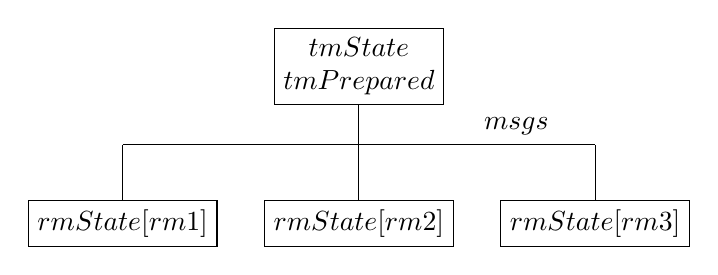
\begin{tikzpicture}[
            >=stealth,
            ent/.style={draw, rectangle, align=center},
            pnt/.style={circle, fill, inner sep=0.15em}
        ]
           \node[ent] at (0,2)(tm) {$tmState$ \\ $tmPrepared$};


           \node[ent] (rm1) at (-3,0) {$rmState[rm1]$};
           \node[ent] (rm2) at (0,0) {$rmState[rm2]$};
           \node[ent] (rm3) at (3,0) {$rmState[rm3]$};

           \draw (-3,1) -- (0,1) -- (3,1);
           \draw (rm1) -- (-3,1);
           \draw (rm2) -- (tm);
           \draw (rm3) -- (3,1);
           \node[above] (msgs) at (2,1) {$msgs$};
        \end{tikzpicture}
    }\end{center}

\end{frame}

\begin{frame}
    \frametitle{Refining the specification}

    The specification for this model is
    \begin{tlabox}
        TPSpec \defeq TPInit \land \Box [TPNext\,]_{\langle
        rmState,\, tmState,\, tmPrepared,\, msgs \rangle}
    \end{tlabox}

    Now we want to check if $TPSpec$ implements $TCSpec$, so we import the
    definitions from module $TCommit$
    \begin{tlabox}
        \INSTANCE TCommit \textcolor{gray!50}{\WITH rmState \leftarrow rmState}
    \end{tlabox}
    and check that \alert{$TPSpec \implies TCSpec$} with TLC.

    \begin{center}
        \scriptsize
        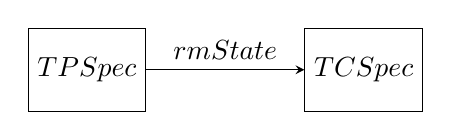
\begin{tikzpicture}[
            >=stealth,
            block/.style={draw, rectangle,
                            minimum height=3em, minimum width=3em}
        ]

            \node[block] (tp) {$TPSpec$};
            \node[block, right of=tp, node distance=10 em] (tc) {$TCSpec$};

            \draw[draw,->] (tp) -- node[above] {$rmState$} (tc);

        \end{tikzpicture}
    \end{center}

\end{frame}

\begin{frame}
    \frametitle{A common step}

    \begin{tlabox}
        TPSpec \defeq TPInit \land \Box [TPNext\,]_{\langle
        rmState,\, tmState,\, tmPrepared,\, msgs \rangle}
    \end{tlabox}

    {\scriptsize
    \setlength\abovedisplayskip{0pt}
    \setlength\belowdisplayskip{0pt}
    \begin{alignat*}{2}
        &\begin{bmatrix}
            tmState : \str{init} \\
            tmPrepared : \{\} \\
            msgs : \{\} \\
            rmState[rm1] : \str{work.}
        \end{bmatrix}
        &\xrightarrow{RMPrepare(rm1)}&
        \begin{bmatrix}
            tmState : \str{init} \\
            tmPrepared : \{\} \\
            \alert{
            msgs = \{[type :\str{Prep}, rm : rm1]\}} \\
            \alert{
            rmState[rm1] : \str{prep.}}
        \end{bmatrix}
        \\[\baselineskip]
        &\begin{bmatrix}
            rmState[rm1] : \str{work.} \\
        \end{bmatrix}
        &\xrightarrow{\phantom{R}Prepare(rm1)\phantom{M}}&
        \begin{bmatrix}
            \phantom{msgs \ \ }
            \alert{
            rmState[rm1] : \str{prep.}}
            \phantom{msgs \ \ }
        \end{bmatrix}
    \end{alignat*}
    }

    \begin{tlabox}
        TCSpec \defeq TCInit \land \Box [TCNext\,]_{rmState}
    \end{tlabox}

\end{frame}

\begin{frame}
    \frametitle{A stutter step}

    \begin{tlabox}
        TPSpec \defeq TPInit \land \Box [TPNext\,]_{\langle
        rmState,\, tmState,\, tmPrepared,\, msgs \rangle}
    \end{tlabox}

    {\scriptsize
    \setlength\abovedisplayskip{0pt}
    \setlength\belowdisplayskip{0pt}
    \begin{alignat*}{2}
        &\begin{bmatrix}
            tmState : \str{init} \\
            tmPrepared : \{\} \\
            msgs = \{\dots\} \\
            rmState[rm1] : \str{prep.}
        \end{bmatrix}
        &\xrightarrow{TMRcvPrepared(rm1)}&
        \begin{bmatrix}
            tmState : \str{init} \\
            \alert{
            tmPrepared : \{rm1\}} \\
            msgs : \{\dots\} \\
            rmState[rm1] : \str{prep.}
        \end{bmatrix}
        \\[\baselineskip]
        &\begin{bmatrix}
            rmState[rm1] : \str{prep.}
        \end{bmatrix}
        &\xrightarrow{\phantom{T} \UNCHANGED rmState \phantom{T}}&
        \begin{bmatrix}
            rmState[rm1] : \str{prep.} \\
        \end{bmatrix}
    \end{alignat*}
    }

    \begin{tlabox}
        TCSpec \defeq TCInit \land \Box [TCNext\,]_{rmState}
    \end{tlabox}

\end{frame}

\begin{frame}
    \frametitle{Taking advantage of symmetry}

    TLC is an explicit-state model checker, so it suffers from state
    explosion. Consider the following possible states according to $TPSpec$:

    {\setlength\abovedisplayskip{0pt}
    \setlength\belowdisplayskip{0pt}
    \begin{gather*}
        s =
        \begin{bmatrix}
            rmState[\textcolor{redPolimi}{rm1}] : \str{prep.} \\
            rmState[\textcolor{bluePolimi}{rm2}] : \str{prep.} \\
            rmState[\textcolor{yellowPolimi}{rm3}] : \str{com.} \\
            \dots
        \end{bmatrix}
        \quad
        s^{\pi} =
        \begin{bmatrix}
            rmState[\textcolor{yellowPolimi}{rm3}] : \str{prep.} \\
            rmState[\textcolor{bluePolimi}{rm2}] : \str{prep.} \\
            rmState[\textcolor{redPolimi}{rm1}] : \str{com.} \\
            \dots
        \end{bmatrix} \\
        \pi = [
            rm1 \mapsto rm3,\,
            rm2 \mapsto rm2,\,
            rm3 \mapsto rm1
        ]
    \end{gather*}}

    Since permutations such as $\pi$ are irrelevant for us, we can take
    advantage of \emph{symmetry}.

\end{frame}

\begin{frame}
    \frametitle{Taking advantage of symmetry}

    \begin{block}{Symmetric specification}
        \setlength\belowdisplayskip{0pt}
        A specification $Spec$ is symmetric with respect to a permutation $\pi$
        over a set of values $S$ if and only if for each behavior $\sigma$:
        \[
             \sigma \models Spec \iff \sigma^{\pi} \models Spec
        \]
    \end{block}

    $TPSpec$ is indeed symmetric w.r.t. the permutations of set $RM$,
    since all resource managers are equal.

    After stating that \alert{$RM$ is a symmetry set} in our model, if TLC
    has already visited a state $s$, it will avoid visiting a state $s^{\pi}$,
    where $\pi$ is a permutation of values in $RM$.

    A reduction of a factor $\lvert RM \rvert !$ can be observed for the number
    of states to be checked.

\end{frame}

\setbeamercovered{invisible}


    \hidesecheadtrue

    \section*{Conclusions}
\begin{frame}{Conclusions}
    \begin{columns}[t]
        \begin{column}{0.5\textwidth}
            \textbf{Pros}
            \begin{itemize}
                \item Quick start with Lamport's video lectures %TODO ref
                \item Focus on abstractions
                \item Good tooling support
                \item Helpful community and material
                \item Actively maintained
            \end{itemize}
        \end{column}
        \begin{column}{0.5\textwidth}
            \textbf{Cons}
            \begin{itemize}
                \item It's math, not programming
                \item Internals are not perfectly documented
            \end{itemize}
        \end{column}
        \end{columns}
\end{frame}

\begin{frame}{Useful Links}
    \begin{itemize}
        \item \tlap website\\
        \smallurl{https://lamport.azurewebsites.net/tla/tla.html}
        \item \tlap tools repository\\
        \smallurl{https://github.com/tlaplus/tlaplus}
        \item \tlap examples\\
        \smallurl{https://github.com/tlaplus/Examples}
        \item Discussion group for users of \tlap\\
        \smallurl{https://groups.google.com/forum/\#!forum/tlaplus}
        \item \tlap specifications for the consistency levels of Azure Cosmos DB\\
        \smallurl{https://github.com/Azure/azure-cosmos-tla}
    \end{itemize}
\end{frame}


    \section*{\texorpdfstring{\Circle}{Next}, \emph{Questions?}}
    \begin{frame}
        \sectionpage
    \end{frame}

    \nocite{*}
    \section*{References}
    \begin{frame}{References}
        \scriptsize
        \bibliographystyle{abbrv}
        \bibliography{references}
    \end{frame}

\end{document}
